\documentclass[varwidth=true, border=2pt]{standalone}
\usepackage{amsmath,amssymb}% math symbols / fonts
\usepackage{tikz}
\usepackage{tqft}
\usetikzlibrary{patterns}

\begin{document}
    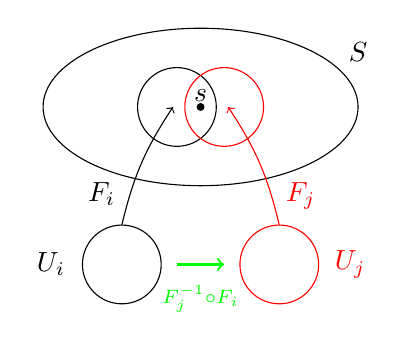
\begin{tikzpicture}
        \tikzstyle{point}=[circle,thick,draw=black,fill=black,inner sep=0pt,minimum width=2pt,minimum height=2pt]
        \draw (0,0) ellipse (2cm and 1cm);
        \def\ringa{(-0.3,0) circle (0.5cm)}
        \def\ringb{(+0.3,0) circle (0.5cm)}

        \draw \ringa;
        \draw[red] \ringb;

        %\node at (-1,0.3) {$U_i$};
        %\node at (+1,0.3) {$U_j$};
        \node at (-1.9,-2) {$U_i$};
        \node[red] at (+1.9,-2) {$U_j$};
        \node at (+2.0,0.7) {$S$};
        \node[point,label={[label distance=-0.1cm]90:$s$}] at (0,0) {};


        \path[<-] (-0.35,0)  edge [bend angle=10,bend right] node[label={[label distance=0.1cm]210:$F_i$}] {} (-1,-1.5);
        \path[<-,red] (+0.35,0)  edge [bend angle=10,bend left]  node[label={[label distance=0.1cm]-30:$F_j$}] {} (+1,-1.5);

        \draw (-1,-2) circle (0.5cm);
        \draw[red] (+1,-2) circle (0.5cm);

        \path[->, green, thick] (-0.3,-2) edge node[label=below:$\scriptstyle F_j^{-1} \circ F_i$] {} (0.3,-2);
    \end{tikzpicture}
\end{document}
